\documentclass{beamer}
\usepackage{tut}

\def\tuttitle{Prolog}
\date{2016-12-12/13}

\prolog

\begin{document}
\normalsize
\normalem

\begin{frame}[plain]
  \titlepage
\end{frame}

\begin{frame}
  \frametitle{Vier Farben}
  Nach dem Vier-Farben-Satz kann jede beliebige Landkarte mit nur vier Farben so gefärbt werden,
  dass keine zwei aneinandergrenzenden Gebiete die gleiche Farbe bekommen.
  In dieser Aufgabe soll eine solche Belegung für die Telefonvorwahlbereiche in Deutschland gefunden werden.
  \begin{figure}
    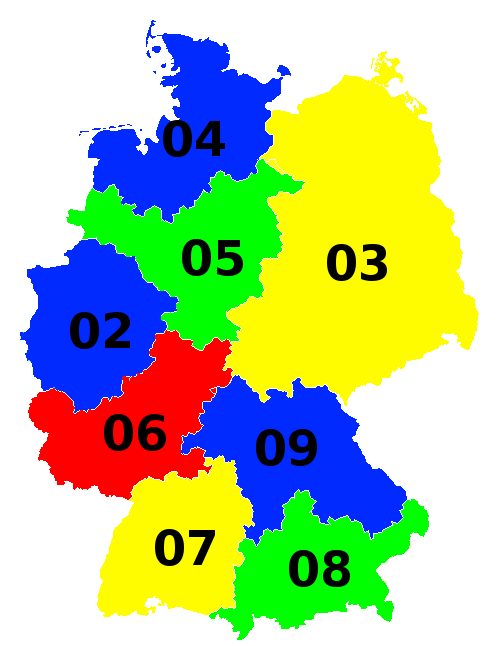
\includegraphics[height=0.5\textheight]{tut7-deutschland}
  \end{figure}
\end{frame}

\begin{frame}[fragile]
  \frametitle{Vier Farben}
  Definiere Prädikat \lstinline{farbe}, welches die vier zu verwendenden Farben festlegt.
  \pause
  \begin{lstlisting}
    farbe(gruen).
    farbe(gelb).
    farbe(blau).
    farbe(rot).
  \end{lstlisting}
  (In SWI-Prolog kann man auch Umlaute verwenden.)
\end{frame}

\begin{frame}[fragile]
  \frametitle{Vier Farben}
  Definiere Prädikat \lstinline{nachbar(X,Y)}, welches erfüllt ist,
  wenn Länder der Farben \lstinline{X} und \lstinline{Y} Nachbarn sein dürfen,
  d.\,h., wenn \lstinline{X} und \lstinline{Y} unterschiedliche Farben sind.
  (Hinweis: wir wollen uns später eine Lösung \emph{generieren} lassen,
  also muss das Prädikat auch für uninstanziierte Variablen funktionieren.)
  \pause
  \begin{lstlisting}
    nachbar(X, Y) :- farbe(X), farbe(Y), X \= Y.
  \end{lstlisting}
\end{frame}

\begin{frame}[fragile]
  Definiere Prädikat \lstinline{deutschland},
  welches Topologie der Karte der 8~Vorwahlbereiche in Deutschland beschreibt.
  \begin{figure}
    \begin{subfigure}{0.3\textwidth}
      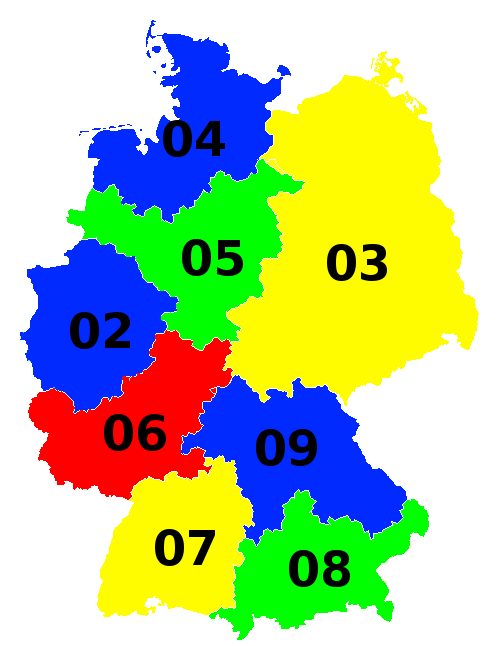
\includegraphics[height=0.5\textheight]{tut7-deutschland}
    \end{subfigure}
    \pause
    \begin{subfigure}{0.65\textwidth}
      \begin{lstlisting}
        deutschland(
          V2, V3, V4, V5,
          V6, V7, V8, V9) :-
         nachbar(V2,V5), nachbar(V2,V6),
         nachbar(V3,V4), nachbar(V3,V5),
           nachbar(V3,V6), nachbar(V3,V9),
         nachbar(V4,V5),
         nachbar(V5,V6),
         nachbar(V6,V7), nachbar(V6,V9),
         nachbar(V7,V8), nachbar(V7,V9),
         nachbar(V8,V9).
      \end{lstlisting}
    \end{subfigure}
  \end{figure}
\end{frame}

\begin{frame}[fragile]
  \frametitle{Vier Farben}
  Wie erhält man nun gültige Einfärbung der Karte?
  \pause
  \begin{lstlisting}
    ?- deutschland(V2,V3,V4,V5,V6,V7,V8,V9).
    V2 = V3, V3 = V7, V7 = gruen,
    V4 = V6, V6 = V8, V8 = blau,
    V5 = V9, V9 = gelb .
  \end{lstlisting}
\end{frame}

\begin{frame}
  \frametitle{Vier Farben}
  Wie findet man heraus, ob die Karte auch nur mit drei Farben färbbar ist?
  
  \pause
  Einen der \lstinline{farbe}-Fakten entfernen und Anfrage erneut stellen.
  
  \pause
  Alternativ: feststellen, dass auch mit vier \lstinline{farbe}-Fakten eine Lösung mit nur drei Farben herauskam.
\end{frame}

\end{document}
